\documentclass[russian, 12pt]{beamer}
\usepackage{multicol}
\usepackage[T2A,T1]{fontenc}
\usepackage[utf8]{inputenc}
\setcounter{secnumdepth}{3}
\setcounter{tocdepth}{3}
\usepackage{amsmath}
\usepackage{amssymb}
\usepackage{graphicx}
\usepackage{paratype}
\usepackage{hyperref}
\usepackage{xcolor}
\usepackage{listings}

\definecolor{codegreen}{rgb}{0,0.6,0}
\definecolor{codegray}{rgb}{0.5,0.5,0.5}
\definecolor{codepurple}{rgb}{0.58,0,0.82}
\definecolor{backcolour}{rgb}{0.95,0.95,0.92}

\lstdefinestyle{mystyle}{
    backgroundcolor=\color{backcolour},   
    commentstyle=\color{codegreen},
    keywordstyle=\color{magenta},
    numberstyle=\tiny\color{codegray},
    stringstyle=\color{codepurple},
    basicstyle=\ttfamily\footnotesize,
    breakatwhitespace=false,         
    breaklines=true,                 
    captionpos=b,                    
    keepspaces=true,                 
    numbers=left,                    
    numbersep=5pt,                  
    showspaces=false,                
    showstringspaces=false,
    showtabs=false,                  
    tabsize=2
}

\newcommand{\R}{\mathbb{R}}
\newcommand{\A}{\mathcal{A}}
\newcommand{\red}[1]{\textcolor{red!85!black}{{#1}}}
\renewcommand{\sp}[1]{\mathrm{sp}\left\{{{#1}}\right\}}
% Syntax: \colorboxed[<color model>]{<color specification>}{<math formula>}
\newcommand*{\colorboxed}{}
\def\colorboxed#1#{%
  \colorboxedAux{#1}%
} 
\newcommand*{\colorboxedAux}[3]{%
  % #1: optional argument for color model
  % #2: color specification
  % #3: formula
  \begingroup
    \colorlet{cb@saved}{.}%
    \color#1{#2}%
    \boxed{%
      \color{cb@saved}%
      #3%
    }%
  \endgroup
}

\makeatletter
\usepackage{tikz}
\usetikzlibrary{overlay-beamer-styles}
\usepackage{pgfplots}
% Remove warning about running in backwards compatibility mode
\pgfplotsset{compat=1.17}
\usepackage[all,cmtip]{xy}
\usetheme{Pittsburgh}
\usefonttheme{professionalfonts}

\setbeamertemplate{navigation symbols}{%
  \hspace{3.8em}%
  \vspace{0.5em}%
  \usebeamercolor[fg]{structure}%
  \usebeamerfont{subtitle}%
  \insertframenumber%
}
\makeatother
\setbeamercovered{invisible}

\usepackage{babel}

\title{Введение. Основные понятия.}
\subtitle{Алгоритмы и структуры данных}
\author{
  Мулюгин Николай
  %\and
  %Кузнецов Максим \texorpdfstring{\thinspace}{Lg}А.
  }
\date{03.09.2022}

\begin{document}

\begin{frame}
\titlepage
\end{frame}
%%%%%%%%%%%%%%%%%%%%%%%%%%%%%%%%%%%%%%%%%%%%%%%%%%%%%%%%%%%%%%%%%%%%%%%%%%%%%%%
\begin{frame}
\frametitle{Информационные источники}
  \begin{itemize}
    \item [1] А. В. Столяров. Введение в профессию.\\
      http://stolyarov.info\\[0.5cm]

    \item [2] К. Владимиров.\\
    youtube.com/channel/UCvmBEbr9NZt7UEh9doI7$\_$A\\[0.5cm]

    \item [3] Ю. Окуловский.\\ 
    https://ulearn.me/

  \end{itemize}
\end{frame}
%%%%%%%%%%%%%%%%%%%%%%%%%%%%%%%%%%%%%%%%%%%%%%%%%%%%%%%%%%%%%%%%%%%%%%%%%%%%%%%
\begin{frame}
\frametitle{Информационные источники}
  \begin{itemize}
    \item [4] Томас Х. Кормен. Алгоритмы: построение и анализ.\\[0.5cm]

    \item [5] Томас Х. Кормен. Алгоритмы. Вводный курс.\\[0.5cm]

    \item [6] Род Стивенс. Алгоритмы. Теория и практическое применение.\\[0.5cm]
    
    \item [7] Никлаус Вирт. Алгоритмы и структуры данных.\\[0.5cm]
    
    \item [8] Д. Кнут. Искусство программирования.

  \end{itemize}
\end{frame}
%%%%%%%%%%%%%%%%%%%%%%%%%%%%%%%%%%%%%%%%%%%%%%%%%%%%%%%%%%%%%%%%%%%%%%%%%%%%%%%
\begin{frame}
\frametitle{Мотивация}
  \begin{itemize}
    \item Применение в науке.\\[0.5cm]

    \item Трудоустройство. Вопросы на собеседовании.\\[0.5cm]

    \item Общение с коллегами.\\[0.5cm]
    
    \item Повседневное применение.\\[0.5cm]

  \end{itemize}
\end{frame}
%%%%%%%%%%%%%%%%%%%%%%%%%%%%%%%%%%%%%%%%%%%%%%%%%%%%%%%%%%%%%%%%%%%%%%%%%%%%%%%
\begin{frame}
\frametitle{Алгоритм}
\textbf{Алгоритм} представляет собой набор правил преобразования исходных данных(input) 
в выходные(output).\\[0.2cm]
\pause
Алгоритмы строятся для решения \textbf{вычислительных задач}.\\[0.2cm]
\pause
\textbf{Свойства} алгоритма:\\[0.2cm]
обязательные \hspace{3cm} необязательные
\begin{multicols}{2}
\begin{itemize}
  \item<4-> [1] Конечность.\\[0.3cm]

  \item<5-> [2] Дискретность.\\[0.3cm]

  \item<6-> [3] Определенность.\\[0.3cm]
  
  \item<7-> [4] Правильность. \\[0.3cm]
  
  \item<8-> [5] Завершаемость. \\[0.3cm]
  
  \item<9-> [6] Массовость. \\

\end{itemize}
\end{multicols}
\end{frame}
%%%%%%%%%%%%%%%%%%%%%%%%%%%%%%%%%%%%%%%%%%%%%%%%%%%%%%%%%%%%%%%%%%%%%%%%%%%%%%%
\begin{frame}
  \frametitle{Сложность алгоритма мотивация}
  Есть алгоритм. Что дальше?\\[0.3cm]
  \pause
  \begin{itemize}

    \item Анализировать алгоритм.\\[0.5cm]
    \pause
    \item Сравнивать различные алгоритмы.\\[0.5cm]
    \pause
    \item Понять как поведет себя алгоритм в будущем.\\[0.5cm]
    
  \end{itemize}
  
  \end{frame}
%%%%%%%%%%%%%%%%%%%%%%%%%%%%%%%%%%%%%%%%%%%%%%%%%%%%%%%%%%%%%%%%%%%%%%%%%%%%%%%
\begin{frame}
\frametitle{Сложность алгоритма}
\textbf{Время работы} алгоритма - 
число элементарных операций, которые он выполняет.\\[0.3cm]
\pause
\textbf{Время работы алгоритма в худшем случае (временная сложность)} - 
максимальное время работы для входов данного размера. \\[0.3cm]
\pause
\textbf{Емкостная сложность} - 
максимально используемый объем памяти для входов данного размера. \\[0.3cm]
\pause
\textbf{Асимптотическая сложность алгоритма} - 
оценка, характеризующая вид зависимости времени работы алгоритма от длины входа.

\end{frame}
%%%%%%%%%%%%%%%%%%%%%%%%%%%%%%%%%%%%%%%%%%%%%%%%%%%%%%%%%%%%%%%%%%%%%%%%%%%%%%%
\lstset{style=mystyle}
\begin{frame}
\frametitle{Сложность алгоритма}
\lstinputlisting[language=C++]{code/complex_1.cpp}
\end{frame}
%%%%%%%%%%%%%%%%%%%%%%%%%%%%%%%%%%%%%%%%%%%%%%%%%%%%%%%%%%%%%%%%%%%%%%%%%%%%%%%
\lstset{style=mystyle}
\begin{frame}[fragile]
\frametitle{Сложность алгоритма}
Посчитаем сложность алгоритма - функцию $f: N\rightarrow N$ которая 
на вход берет n - длину входа и возвращает
число элементарных операций для данного n.\\[0.3cm]
\begin{lstlisting}[language=C++]
int n = input.size();
int sum = 0;
for( int i = 0; i < n; i++ )
    for( int j = 0; j < 2 * i; j++ )
        sum++; 
\end{lstlisting}
\end{frame}
%%%%%%%%%%%%%%%%%%%%%%%%%%%%%%%%%%%%%%%%%%%%%%%%%%%%%%%%%%%%%%%%%%%%%%%%%%%%%%%
\lstset{style=mystyle}
\begin{frame}[fragile]
\frametitle{Сложность алгоритма}
\begin{lstlisting}[language=C++]
int n = input.size();
int sum = 0;
for( int i = 0; i < n; i++ )//n
    for( int j = 0; j < 2 * i; j++ )
    //01 0123 012345 0123456 012..2i-1
        sum++;//0 + 2 + 4 + 6 + ... 2(n-1)  
\end{lstlisting}
$f(n) = n \cdot (C_= + C_< + C_* + C_+) +$\\
$ + 2\cdot n \cdot (n-1) \cdot (C_= + C_< + C_* + C_+) + C_{in} + C_{out}$\\[0.3cm]
f(n) - характеристика нашего алгоритма. \\
Какие выводы мы можем сделать по ней?
\end{frame}
%%%%%%%%%%%%%%%%%%%%%%%%%%%%%%%%%%%%%%%%%%%%%%%%%%%%%%%%%%%%%%%%%%%%%%%%%%%%%%%
\begin{frame}
  \frametitle{Сложность алгоритма мотивация}
  \begin{itemize}
    \item Анализировать алгоритм.\\[0.5cm]
    
    \item Сравнивать различные алгоритмы.\\[0.5cm]
  
    \item Понять как поведет себя алгоритм в будущем.\\[0.5cm]
    
  \end{itemize}
  
  \end{frame}
%%%%%%%%%%%%%%%%%%%%%%%%%%%%%%%%%%%%%%%%%%%%%%%%%%%%%%%%%%%%%%%%%%%%%%%%%%%%%%%
\begin{frame}
\frametitle{Переменные}

\begin{center}
\begin{tikzpicture}
    \draw<1-3> (0,0) rectangle (1.8, 0.6);
    \draw<1-3> (0.9,0.3) node[scale=1.5] {0100};
    
    %2
    \draw<2-3> (-1, 1.5) node[scale=2, color=blue] {a};
    \draw<2-3> (0.5, 1.5) node[scale=1.7, color=blue] {4};
    \draw<2-3> (2.5, 1.5) node[scale=1.5, color=blue] {[-7$\div$8]};
    %3
    \draw<3-> (1, -1) node[scale=1.2] {Мы знаем тип а?};
    %4
    \draw<3-> (1, -2) node[scale=1.2] {Мы знаем диапозон значений!};
    %5
    \draw<4-> (-3,0) rectangle (-1.2, 0.6);
    \draw<4-> (-2.1,0.3) node[scale=1.5] {0100};

    \draw<4-> (3,0) rectangle (4.8, 0.6);
    \draw<4-> (3.9,0.3) node[scale=1.5] {0011};

    \draw<4-> (1, -3) node[scale=1.2] {Мы не знаем операции!};
    \draw<4-> (-3, 1.5) node[scale=2, color=blue] {a};
    \draw<4-> (-1.5, 1.5) node[scale=1.7, color=blue] {4};

    \draw<4-> (0.8, 1.5) node[scale=1.5, color=blue] {[-7$\div$8]};
    \draw<4-> [dashed] (-1.2, 0.6) -- (0, 1.3);
    \draw<4-> [dashed] (3, 0.6) -- (1.6, 1.3);

    \draw<4-> (3, 1.5) node[scale=1.7, color=blue] {4};
    \draw<4-> (4.5, 1.5) node[scale=1.5, color=blue] {b};

    
\end{tikzpicture}
\end{center}

\end{frame}
%%%%%%%%%%%%%%%%%%%%%%%%%%%%%%%%%%%%%%%%%%%%%%%%%%%%%%%%%%%%%%%%%%%%%%%%%%%%%%%
\begin{frame}
\frametitle{Типы}

\begin{itemize}
  \item Что такое тип?\\[0.3cm]
  \item value type: диапозон значений объекта\\[0.3cm]
  \item object type: совокупность операций над объектом\\[0.15cm]
  \begin{itemize}
    \item 5/2 даст 2 для int но 2.5 для double\\[0.2cm]
  \end{itemize}

  \item Назовем целочисленный арифметический тип i4
\end{itemize}

\end{frame}
%%%%%%%%%%%%%%%%%%%%%%%%%%%%%%%%%%%%%%%%%%%%%%%%%%%%%%%%%%%%%%%%%%%%%%%%%%%%%%%
\begin{frame}
\begin{center}
\begin{tikzpicture}
  \draw<-4> (-3,0) rectangle (-1.2, 0.6);
  \draw<5-> (-4,0) rectangle (5.5, 0.6);
  \draw (-2.1,0.3) node[scale=1.5, color=blue] {0100};

  \draw<5-> (-3.4,0.3) node[scale=1.5] {110};
  \draw<5-> (0.9,0.3) node[scale=1.5] {1000110010111};
  \draw<5-> (5,0.3) node[scale=1.5] {01};

  \draw<-4> (3,0) rectangle (4.8, 0.6);
  \draw (3.9,0.3) node[scale=1.5, color=blue] {0011};

  \draw (-3, 1.5) node[scale=2, color=blue] {a};
  \draw<-4> (-1.5, 1.5) node[scale=1.7, color=blue] {4};

  \draw<-2> (0.8, 1.5) node[scale=1.5, color=blue] {i4};
  \draw<-2> [dashed] (-1.2, 0.6) -- (0.5, 1.3);
  \draw<-2> [dashed] (3, 0.6) -- (1.1, 1.3);

  \draw<-4> (3, 1.5) node[scale=1.7, color=blue] {3};
  \draw (4.5, 1.5) node[scale=1.5, color=blue] {b};
  %2
  \draw<2> (0.8, 2) node[scale=1, color=blue] {python};
  \draw<2> (0.8, 2.5) node[scale=1, color=blue] {ruby};
  %3
  \draw<3-7> (0.8, 2.5) node[scale=1.5, color=blue] {i4};
  \draw<3-7> [dashed] (-2.7, 1.7) -- (0.5, 2.5);
  \draw<3-7> [dashed] (4.2, 1.7) -- (1.1, 2.5);

  \draw<3-> [dashed] (-2.7, 1.3) -- (-2.5, 0.7);
  \draw<3-> [dashed] (4.2, 1.3) -- (4, 0.7);
  \draw<4> (0.8, -2) node[scale=1] {Имя навсегда связано с типом.};
  %\draw<4-> (0.8, 3) node[scale=1, color = blue] {c++};
  \draw<4> (0.8, 3) node[scale=1, color = blue] {java};
  \draw<4> (0.8, 3.5) node[scale=1, color = blue] {c$\#$};
  \draw<5> (0.8, 3) node[scale=1, color = blue] {c};
  %6
  \draw<6->[dashed] (-2.6,0) -- (-2.6,-1);
  \draw<6->[dashed] (-3.7,0) -- (-3.7,-1.5);
  \draw<6->[dashed] (3.4,0) -- (3.4,-1.5);

  \draw<6-> (-3.6,-1.3)--(3.3,-1.3);
  \draw<6-> (-3.6,-0.4)--(-2.7,-0.4);

  \draw<6-> (-3, -0.6) node[scale=1] {$\&$a};
  \draw<6-> (0, -1.6) node[scale=1] {$\&$b};
  %7
  \draw<7->[dashed, color=red] (-3, -0.8) -- (-2.6,-3);
  \draw<7->[dashed, color=red] (-2.4,-3) -- (-0.1, -1.8);
  \draw<7-> (-2.6, -3.3) node[scale=1] {i4*};
  \draw<7> (4, -3.3) node[scale=1] {Какой размер типа i4* ?};
  \draw<7> (4, -4) node[scale=1] {Какое значение CHAR$\_$BIT ?};
  %8
  \draw<8-> (-0.132,0.3) node[scale=1.51, color=red] {00011};
  \draw<8>[->, line width=0.5mm, color=orange]  (-0.2,-0) to[out=-0,in=-40] (-2.6, 0);

  \draw<8> (0.6, 1.7) node[scale=1.5, color=red] {pa};
  \draw<8> [dashed,color=red] (0, 0.7) -- (0.5, 1.5);

  \draw<8> (1.6, 2.4) node[scale=1] {i4* [0$\div$26]};
  \draw<8> [dashed] (1, 1.8) -- (1.4, 2.2);
  \draw<8> (-1.4, -0.5) node[scale=0.7] {points-to};
  \draw<5> (-1.4, -1) node[scale=1.2] {RAM - random access memory};



\end{tikzpicture}
\end{center}

\end{frame}
%%%%%%%%%%%%%%%%%%%%%%%%%%%%%%%%%%%%%%%%%%%%%%%%%%%%%%%%%%%%%%%%%%%%%%%%%%%%%%%
\begin{frame}
\frametitle{Указатели}
\begin{itemize}
  \item Если указатель это просто расстояние, то может быть нулевое расстояние?
    \begin{itemize}
      \item nullptr
    \end{itemize}
  \item p[2] == *(p+2)
\end{itemize}
\end{frame}
%%%%%%%%%%%%%%%%%%%%%%%%%%%%%%%%%%%%%%%%%%%%%%%%%%%%%%%%%%%%%%%%%%%%%%%%%%%%%%%
\begin{frame}
  \begin{center}
  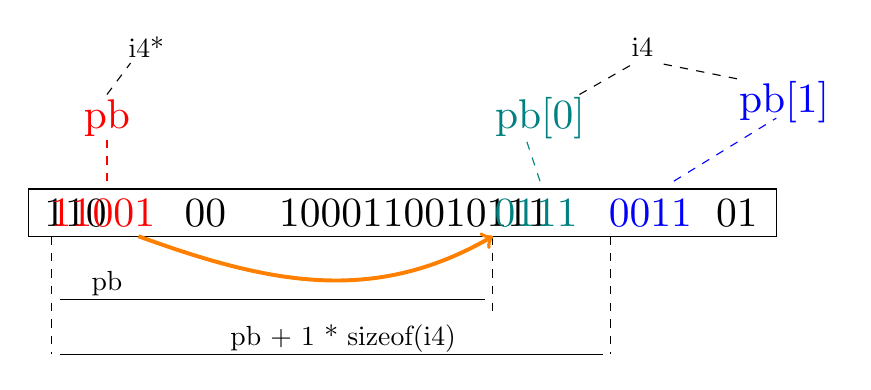
\begin{tikzpicture}
    \draw (-4,0) rectangle (5.5, 0.6);
    \draw (-1.75,0.3) node[scale=1.5] {00};
  
    \draw (-3.4,0.3) node[scale=1.5] {110};
    \draw (0.9,0.3) node[scale=1.5] {1000110010111};
    \draw (5,0.3) node[scale=1.5] {01};
  
    \draw (2.45,0.3) node[scale=1.5, color=teal] {0111};
    \draw (3.9,0.3) node[scale=1.5, color=blue] {0011};
    \draw (-3, 1.5) node[scale=1.5, color=red] {pb};
    \draw (2.5, 1.5) node[scale=1.5, color=teal] {pb[0]};
    \draw[dashed] (1.9,0) -- (1.9,-1);
    \draw[dashed] (-3.7,0) -- (-3.7,-1.5);
    \draw[dashed] (3.4,0) -- (3.4,-1.5);
  
    \draw (-3.6,-1.5)--(3.3,-1.5);
    \draw (-3.6,-0.8)--(1.8,-0.8);
  
    \draw (-3, -0.6) node[scale=1] {pb};
    \draw (0, -1.3) node[scale=1] {pb + 1 * sizeof(i4)};
  
    %8
    \draw (-3.05,0.3) node[scale=1.51, color=red] {11001};
    \draw[->, line width=0.5mm, color=orange]  (-2.6, 0) to[out=-20,in=-150] (1.9,-0);
  
    \draw (5.6, 1.7) node[scale=1.5, color=blue] {pb[1]};
    \draw[dashed,color=blue] (4.2, 0.7) -- (5.5, 1.5);
  
    \draw (-2.5, 2.4) node[scale=1] {i4*};
    \draw (3.8, 2.4) node[scale=1] {i4};
    \draw [dashed] (3, 1.8) -- (3.7, 2.2);
    \draw [dashed] (5, 2) -- (4, 2.2);
    \draw [dashed,color=teal] (2.5, 0.7) -- (2.3, 1.3);
    \draw [dashed,color=red] (-3, 0.7) -- (-3, 1.3);
    \draw [dashed] (-3, 1.8) -- (-2.7, 2.2);
  
  \end{tikzpicture}
  \end{center}
  
  \end{frame}
%%%%%%%%%%%%%%%%%%%%%%%%%%%%%%%%%%%%%%%%%%%%%%%%%%%%%%%%%%%%%%%%%%%%%%%%%%%%%%%
\begin{frame}
\frametitle{Ссылки}
\begin{itemize}
  \item Два имени у одного объекта в С++.
\end{itemize}
\begin{center}
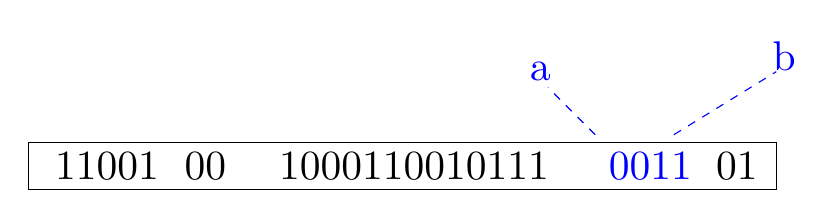
\begin{tikzpicture}
  \draw (-4,0) rectangle (5.5, 0.6);
  \draw (-1.75,0.3) node[scale=1.5] {00};

  \draw (-3,0.3) node[scale=1.5] {11001};
  \draw (0.9,0.3) node[scale=1.5] {1000110010111};
  \draw (5,0.3) node[scale=1.5] {01};
  \draw (3.9,0.3) node[scale=1.5, color=blue] {0011};
  \draw (2.5, 1.5) node[scale=1.5, color=blue] {a};
  \draw (5.6, 1.7) node[scale=1.5, color=blue] {b};
  \draw[dashed,color=blue] (4.2, 0.7) -- (5.5, 1.5);
  \draw [dashed,color=blue] (3.2, 0.7) -- (2.6, 1.3);

\end{tikzpicture}
\end{center}
\end{frame}
%%%%%%%%%%%%%%%%%%%%%%%%%%%%%%%%%%%%%%%%%%%%%%%%%%%%%%%%%%%%%%%%%%%%%%%%%%%%%%%
\begin{frame}[fragile]
\frametitle{Ссылки}
Базовый синтаксис lvalue ссылок это одинарный амперсанд
\begin{lstlisting}
int x;
int &y = x; // y - another name for x
\end{lstlisting}
\pause
Не путать со взятием адреса!
\pause
\begin{columns}[T] % align columns
\begin{column}{.48\textwidth}
  \begin{lstlisting}
  int x[2] = {10, 20};
  int &xref = x[0];
  int *xref = &x[0];
  xref += 1;
  xptr += 1;
  assert(xref == 11);
  assert(xptr == 20);
  \end{lstlisting}
\end{column}%
\hfill%
\begin{column}{.48\textwidth}
  \begin{figure}
    \includegraphics <3>[width=\linewidth, height=3cm]{img/lref_1.png}
    \includegraphics <4>[width=\linewidth, height=3cm]{img/lref_2.png}
  \end{figure}
\end{column}%
\end{columns} 
\end{frame}
%%%%%%%%%%%%%%%%%%%%%%%%%%%%%%%%%%%%%%%%%%%%%%%%%%%%%%%%%%%%%%%%%%%%%%%%%%%%%%%
\lstset{style=mystyle}
\begin{frame}[fragile]
\frametitle{Оценка сложности алгоритма}
Чем мы тут занимаемся???
\begin{lstlisting}[language=C++]
int n = input.size();
int sum = 0;
for( int i = 0; i < n; i++ )//n
  for( int j = 0; j < 2 * i; j++ )
  //01 0123 012345 0123456 012..2i-1
      sum++;//0 + 2 + 4 + 6 + ... 2(n-1)  
\end{lstlisting}
  $f(n) = n \cdot (C_= + C_< + C_* + C_+) +$\\
  $ + 2\cdot n \cdot (n-1) \cdot (C_= + C_< + C_* + C_+) + C_{in} + C_{out}$\\[0.3cm]
  \begin{itemize}
    \item f(n) - характеристика нашего алгоритма.
    \item Какие выводы мы можем сделать по ней?
    %\item<2> $f(n) :\; n \rightarrow \infty$
  \end{itemize}
  
\end{frame}
%%%%%%%%%%%%%%%%%%%%%%%%%%%%%%%%%%%%%%%%%%%%%%%%%%%%%%%%%%%%%%%%%%%%%%%%%%%%%%%
\begin{frame}
\frametitle{Мотивация!!!}
Есть алгоритм. Что дальше?\\[0.3cm]

\begin{itemize}

  \item Анализировать алгоритм.\\[0.5cm]
  
  \item Понять как поведет себя алгоритм в будущем.\\[0.5cm]
  
  \item Сравнивать различные алгоритмы.\\[0.5cm]
  
\end{itemize}

\end{frame}
%%%%%%%%%%%%%%%%%%%%%%%%%%%%%%%%%%%%%%%%%%%%%%%%%%%%%%%%%%%%%%%%%%%%%%%%%%%%%%%
\begin{frame}[fragile]
\frametitle{Анализировать алгоритм}
\begin{lstlisting}[language=C++]
int n = input.size();
int sum = 0;
for( int i = 0; i < n; i++ )//n
  for( int j = 0; j < 2 * i; j++ )
  //01 0123 012345 0123456 012..2i-1
      sum++;//0 + 2 + 4 + 6 + ... 2(n-1)  
\end{lstlisting}
$f(n) = n \cdot (C_= + C_< + C_* + C_+) +$\\
$ + 2\cdot n \cdot (n-1) \cdot (C_= + C_< + C_* + C_+) + C_{in} + C_{out}$\\[0.2cm]
\pause
f(n)- показывает зависимость алгоритма от длины входа.
\end{frame}
%%%%%%%%%%%%%%%%%%%%%%%%%%%%%%%%%%%%%%%%%%%%%%%%%%%%%%%%%%%%
\begin{frame}[fragile]
\frametitle{Понять как поведет себя алгоритм в будущем}
\begin{lstlisting}[language=C++]
int n = input.size();
int sum = 0;
for( int i = 0; i < n; i++ )//n
  for( int j = 0; j < 2 * i; j++ )
  //01 0123 012345 0123456 012..2i-1
      sum++;//0 + 2 + 4 + 6 + ... 2(n-1)  
\end{lstlisting}
$f(n) = n \cdot (C_= + C_< + C_* + C_+) +$\\
$ + 2\cdot n\cdot (n-1) \cdot (C_= + C_< + C_* + C_+) + C_{in} + C_{out}$\\[0.2cm]
\pause
$f(n) :\; n \rightarrow \infty$
\pause
\begin{lstlisting}[language=python]
f(n) = n*(1+1+1+1) + 2*n*(n-1)*(1+1+1+1) + 5 + 5
plot(f, (n,0,100), axes_labels=['n','f(n)']) 
\end{lstlisting}
\end{frame}
%%%%%%%%%%%%%%%%%%%%%%%%%%%%%%%%%%%%%%%%%%%%%%%%%%%%%%%%%%%%
\begin{frame}[fragile]
\frametitle{Понять как поведет себя алгоритм в будущем}
\begin{figure}
  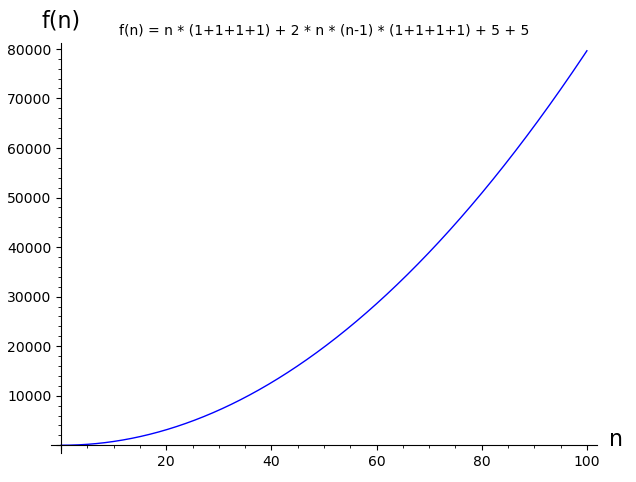
\includegraphics[width=0.8\linewidth, height=5cm]{img/complexity_1.png}
  %\caption{A boat.}
  %\label{fig:boat1}
\end{figure}
\end{frame}
%%%%%%%%%%%%%%%%%%%%%%%%%%%%%%%%%%%%%%%%%%%%%%%%%%%%%%%%%%%%%%%%%%%%%%%%%%%%%%%
\begin{frame}
\frametitle{Масштаб роста фунций}
$f(n) = n \cdot (C_= + C_< + C_* + C_+) +$\\
$ + 2\cdot n\cdot (n-1) \cdot (C_= + C_< + C_* + C_+) + C_{in} + C_{out}=$\\
\pause
$= n \cdot C_1 + 2\cdot n\cdot (n-1) \cdot C_2 + C_3=$\\
\pause
$= 2\cdot n^2 \cdot C_2 + n \cdot(C_1 -2\cdot C_2) + C_3=$\\[0.2cm]
\pause
$= 2\cdot n^2 \cdot C_2 + n \cdot C_4 + C_3.$\\[0.2cm]
\pause
Может быть нам более интеерсен масштаб роста функции?\\[0.2cm]
\pause
Не все ли равно какие коэффициенты $C_1$, $C_2$, $C_3$, $C_4$\\ 
при $n\rightarrow\infty$? 
\end{frame}
%%%%%%%%%%%%%%%%%%%%%%%%%%%%%%%%%%%%%%%%%%%%%%%%%%%%%%%%%%%%%%%%%%%%%%%%%%%%%%%
\begin{frame}[fragile]
\frametitle{Масштаб роста фунций}
\begin{lstlisting}[language=Python]
f(n) = 10*n^2 + n *10 + 10
g(n) = 100*n^2 + n *100 + 100

f_p = plot(f, (n,0,100))
g_p = plot(g, (n,0,100))
ans = f_p + g_p 

ans += text("g(n)", (100, +200000))
ans += text("f(n)", (80, +800000))
ans
\end{lstlisting}
\end{frame}
%%%%%%%%%%%%%%%%%%%%%%%%%%%%%%%%%%%%%%%%%%%%%%%%%%%%%%%%%%%%%%%%%%%%%%%%%%%%%%%
\begin{frame}[fragile]
\frametitle{Масштаб роста фунций}
\begin{figure}
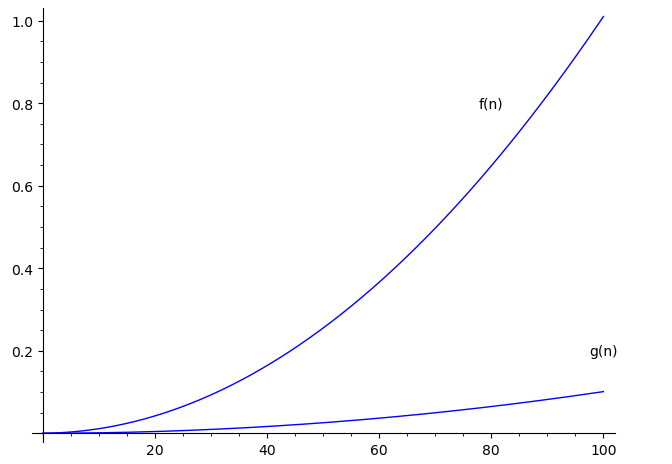
\includegraphics[width=0.8\linewidth, height=5cm]{img/complexity_2.png}
%\caption{A boat.}
%\label{fig:boat1}
\end{figure}
\end{frame}
%%%%%%%%%%%%%%%%%%%%%%%%%%%%%%%%%%%%%%%%%%%%%%%%%%%%%%%%%%%%%%%%%%%%%%%%%%%%%%%
\begin{frame}[fragile]
\frametitle{Масштаб роста фунций}
\begin{lstlisting}[language=Python]
f(n) = 10*n^2 + n *10 + 10
g(n) = 100*n^2 + n *100 + 100

f_p = plot(f, (n,0,100000000))
g_p = plot(g, (n,0,100000000))
ans = f_p + g_p 
ans+= text("g(n)", (80000000, +100000000000000000))
ans+= text("f(n)", (80000000, +900000000000000000))
ans
\end{lstlisting}
\end{frame}
%%%%%%%%%%%%%%%%%%%%%%%%%%%%%%%%%%%%%%%%%%%%%%%%%%%%%%%%%%%%%%%%%%%%%%%%%%%%%%%
\begin{frame}
\frametitle{Масштаб роста фунций}
\begin{figure}
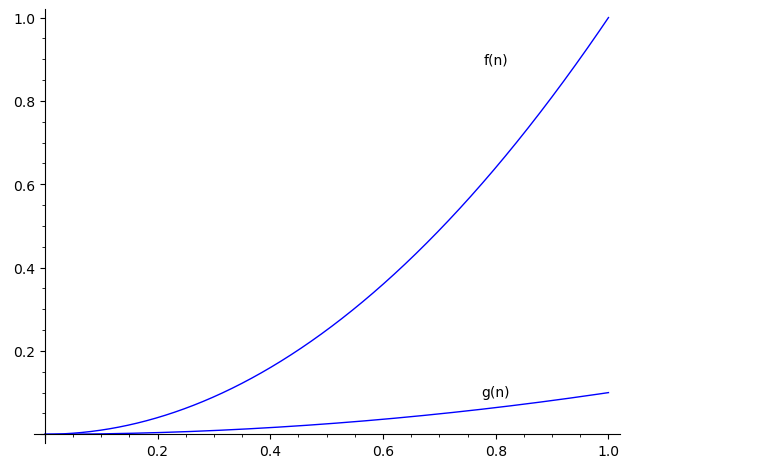
\includegraphics[width=\linewidth, height=5cm]{img/complexity_3.png}
%\caption{A boat.}
%\label{fig:boat1}
\end{figure}
\end{frame}
%%%%%%%%%%%%%%%%%%%%%%%%%%%%%%%%%%%%%%%%%%%%%%%%%%%%%%%%%%%%%%%%%%%%%%%%%%%%%%%
\begin{frame}[fragile]
\frametitle{Масштаб роста фунций}
\begin{lstlisting}[language=Python]
f(n) = 10*n^2 + n *10 + 10
quad(n) = 2*n^2
lin(n) = 1000*n

f_p = plot(f, (n,0,1000))
quad_p = plot(quad, (n,0,1000), color='red')
lin_p = plot(lin, (n,0,1000),color = 'green')
ex_p = plot(ex, (n,0,1000),color = 'brown')

ans = f_p + quad_p + lin_p
ans
\end{lstlisting}
\end{frame}
%%%%%%%%%%%%%%%%%%%%%%%%%%%%%%%%%%%%%%%%%%%%%%%%%%%%%%%%%%%%%%%%%%%%%%%%%%%%%%%
\begin{frame}
\frametitle{Масштаб роста фунций}
\begin{figure}
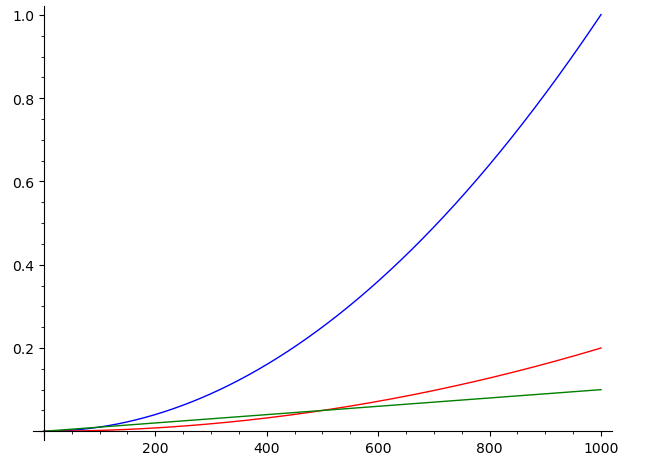
\includegraphics[width=\linewidth, height=5cm]{img/complexity_4.png}
%\caption{A boat.}
%\label{fig:boat1}
\end{figure}
\end{frame}
%%%%%%%%%%%%%%%%%%%%%%%%%%%%%%%%%%%%%%%%%%%%%%%%%%%%%%%%%%%%%%%%%%%%%%%%%%%%%%%
\begin{frame}
\frametitle{Масштаб роста фунций}
\begin{figure}
  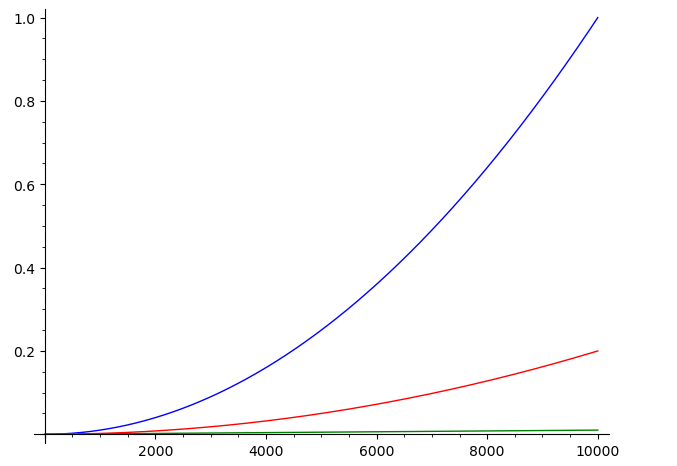
\includegraphics[width=\linewidth, height=5cm]{img/complexity_5.png}
  %\caption{A boat.}
  %\label{fig:boat1}
\end{figure}
\end{frame}
%%%%%%%%%%%%%%%%%%%%%%%%%%%%%%%%%%%%%%%%%%%%%%%%%%%%%%%%%%%%%%%%%%%%%%%%%%%%%%%
\begin{frame}
\frametitle{Масштаб роста фунций}
\begin{figure}
  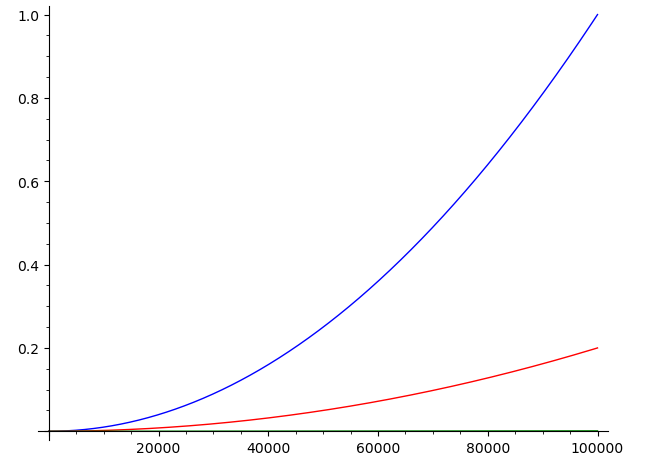
\includegraphics[width=\linewidth, height=5cm]{img/complexity_6.png}
  %\caption{A boat.}
  %\label{fig:boat1}
\end{figure}
\end{frame}
%%%%%%%%%%%%%%%%%%%%%%%%%%%%%%%%%%%%%%%%%%%%%%%%%%%%%%%%%%%%%%%%%%%%%%%%%%%%%%%
\begin{frame}
\frametitle{Масштаб роста фунций}
$f(n) = 2\cdot n^2 \cdot C_2 + n \cdot C_4 + C_3.$\\[0.3cm]
\begin{itemize}
  \pause
  \item Как максимально коротко и точно описать сложность алгоритма?\\[0.3cm]
  \pause
  \item Возьмем самое значимое слагаемое.\\[0.3cm]
  \pause
  \item Можем ли мы подтвердить интуицую математикой?
\end{itemize}
\end{frame}
%%%%%%%%%%%%%%%%%%%%%%%%%%%%%%%%%%%%%%%%%%%%%%%%%%%%%%%%%%%%%%%%%%%%%%%%%%%%%%%
\begin{frame}
\frametitle{O-символика}
%I
\begin{equation*}
\text{f(n) = o(g(n))}
  \begin{array}{l}
  \forall\text{k > 0}\;\exists\text{n}_0\;  \forall \text{n >}\text{n}_0  \\
  \text{f(n) < k $\cdot$ g(n)}
  \end{array}
\Leftrightarrow
\lim_{n\rightarrow\infty}\frac{\text{f(n)}}{\text{g(n)}}=\text{0}
\hspace{0.49cm}
\text{f(n) $\prec$ g(n)}
\end{equation*}
\vspace{0.3cm}
%II
\begin{equation*}
\text{f(n) = O(g(n))}
  \begin{array}{l}
    \exists\text{k > 0}\;\exists\text{n}_0\;  \forall \text{n >}\text{n}_0  \\
    \text{f(n) < k $\cdot$ g(n)}
  \end{array}
\Leftrightarrow
\lim_{n\rightarrow\infty}\frac{\text{f(n)}}{\text{g(n)}}<\infty
\hspace{0.25cm}
\text{f(n) $\preceq$ g(n)}
\end{equation*}
\vspace{0.3cm}
%III
\begin{equation*}
\text{f(n) = $\Theta$(g(n))}
%\hspace{0.2cm}
  \begin{array}{l}
    \exists\text{k}_1\text{k}_2 >\text{0}\;\exists\text{n}_0\hspace{0.5cm}\\
    \forall \text{n >}\text{n}_0\\
    \text{k}_1 \cdot \text{g(n)} < \text{f(n)}\\
    \text{f(n)} < \text{k}_2 \cdot \text{g(n)}
  \end{array}
\hspace{0.2cm}
\Leftarrow
\lim_{n\rightarrow\infty}\frac{\text{f(n)}}{\text{g(n)}}=\text{c}
\hspace{0.4cm}
\text{f(n) $\approx$ g(n)}
\end{equation*}
\end{frame}
%%%%%%%%%%%%%%%%%%%%%%%%%%%%%%%%%%%%%%%%%%%%%%%%%%%%%%%%%%%%%%%%%%%%%%%%%%%%%%%
%\lstset{style=mystyle}
\begin{frame}
  $f(n) = 2\cdot n^2 \cdot C_2 + n \cdot C_4 + C_3.$\\[0.1cm]
  $g(n) = n^2$\\[0.2cm]
  $\lim_{n\rightarrow\infty}\frac{f(n)}{g(n)} =$\pause
  $\lim_{n\rightarrow\infty}\frac{2\cdot n^2 \cdot C_2 + 
  n \cdot C_4 + C_3}{n^2}=$\\[0.3cm]\pause
  $\lim_{n\rightarrow\infty}\frac{2\cdot n^2}{n^2}+
  \lim_{n\rightarrow\infty}\frac{n \cdot C_4}{n^2}+
  \lim_{n\rightarrow\infty}\frac{C_3}{n^2}=$\\[0.3cm]\pause
  $\lim_{n\rightarrow\infty}\frac{2}{1}+
  \lim_{n\rightarrow\infty}\frac{C_4}{n}+
  \lim_{n\rightarrow\infty}\frac{C_3}{n^2}=$\\[0.3cm]\pause
  $2 + 0 + 0 = 2$
\end{frame}
%%%%%%%%%%%%%%%%%%%%%%%%%%%%%%%%%%%%%%%%%%%%%%%%%%%%%%%%%%%%%%%%%%%%%%%%%%%%%%%
\begin{frame}
\frametitle{Классы сложности}
Алгоритм со сложностью f(n) называется:
\begin{itemize}
  \item Если f $=\Theta(\log^kn)$: 
  логарифмическим при k=1, полилогарифмическим при k>1.\\[0.3cm]

  \item Если f $=\Theta(n)$: 
  линейным.\\[0.3cm]

  \item Если f $=\Theta(n\log^kn)$: 
  linearithmic при k=1, квазилинейным при k>1.\\[0.3cm]
  
  \item Если f $=\Theta(n^k)$: 
  полиномиальным, при k=2 квадратическим. \\[0.3cm]
  
  \item Если f $=\Theta(2^{n^k})$: 
  экспоненциальным. \\

\end{itemize}
\end{frame}
%%%%%%%%%%%%%%%%%%%%%%%%%%%%%%%%%%%%%%%%%%%%%%%%%%%%%%%%%%%%%%%%%%%%%%%%%%%%%%%
\lstset{style=mystyle}
\begin{frame}[fragile]
%\lstinputlisting[language=C++]{code/trap_divisor.cpp}
\begin{lstlisting}[language=C++]
#include<iostream> 
#include<string>
#include<cmath>
int main()
{
    int n, root;
    std::cin >> n;
    root = std::sqrt( n );
    for( int i=2;i<=root;i++ ){
        if(n%i == 0){
            std::cout << i << std::endl;
            return 0;
        }
    }
    std::cout << n << " is prime" << std::endl;
    return 0;
}  
\end{lstlisting}
\end{frame}
%%%%%%%%%%%%%%%%%%%%%%%%%%%%%%%%%%%%%%%%%%%%%%%%%%%%%%%%%%%%%%%%%%%%%%%%%%%%%%%
\lstset{style=mystyle}
\begin{frame}[fragile]
%\lstinputlisting[language=C++]{code/trap_divisor.cpp}
\begin{lstlisting}[language=C++]
#include<iostream> 
#include<string>
#include<cmath>
int main()
{
    int n, root;
    std::cin >> n;
    root = std::sqrt( n );
    for( int i=2;i<=root;i++ ){
        if(n%i == 0){//2 3 4 5 ... sqrt(n)
            std::cout << i << std::endl;
            return 0;
        }
    }
    std::cout << n << " is prime" << std::endl;
    return 0;
}  
\end{lstlisting}
\end{frame}
%%%%%%%%%%%%%%%%%%%%%%%%%%%%%%%%%%%%%%%%%%%%%%%%%%%%%%%%%%%%%%%%%%%%%%%%%%%%%%%
\lstset{style=mystyle}
\begin{frame}[fragile]
\begin{columns}[T] % align columns
\begin{column}{.48\textwidth}
\begin{lstlisting}[language=C++]
int n, root;
std::cin >> n;
root = std::sqrt( n );
for(int i=2;i<=root;i++)
\end{lstlisting}
\end{column}%
\hfill%
\begin{column}{.48\textwidth}
$f(n) = \Theta( \sqrt{n} )$\\[0.3cm]
\pause
$n = \Theta( 10^{|x|} )$\\[0.3cm]
\pause
$f(|x|) = \Theta\left( \sqrt{10^{|x|}} \right)$
\end{column}%
\end{columns} 
\end{frame}
%%%%%%%%%%%%%%%%%%%%%%%%%%%%%%%%%%%%%%%%%%%%%%%%%%%%%%%%%%%%%%%%%%%%%%%%%%%%%%%
\begin{frame}
\frametitle{Домашнее задание}
\begin{itemize}
  \item Написать программу реализующую алгоритм Эратосфена.
  \item Оценить сложность - написать в программе комментариями мысли и результат.
  \item Сделать pull request в папку lecture$\_$01/homework/ с файлом решения.
\end{itemize}
\end{frame}


\end{document}
